\documentclass{standalone}
\usepackage{chez}

\begin{document}
\chapter{December 09, 2020}

\section{Homotopy groups of spheres}
Recall that \(\pi_m S^n\) is the group of continuous maps
from \(S^m\) to \(S^n\) up to homotopy.

\begin{theorem}[Freudenthal]
  For \(n \geq k + 2\), \(\pi_{n+k} S^n\) is independent of \(n\).
  This group is denoted \(\pi_k \mathbb S\).
\end{theorem}
\begin{example}
  \(\pi_3 S^2 \iso \ZZ\),
  \(\pi_4 S^3 \iso \ZZ/2\ZZ\),
  \(\pi_5 S^4 \iso \ZZ/2\ZZ\), \dots,
  so \(\pi_1 \mathbb S \iso \ZZ/2\ZZ\).
\end{example}

The first couple of stable groups are
\begin{itemize}[nosep]
  \item \(\pi_1 \mathbb S \iso \ZZ/2\ZZ\)
  \item \(\pi_2 \mathbb S \iso \ZZ/2\ZZ\)
  \item \(\pi_3 \mathbb S \iso \ZZ/8\ZZ \oplus \ZZ/3\ZZ\)
  \item \(\pi_4 \mathbb S \iso 0\)
  \item \(\pi_5 \mathbb S \iso 0\)
  \item \(\pi_6 \mathbb S \iso \ZZ/2\ZZ\)
  \item \(\pi_7 \mathbb S \iso \ZZ/16\ZZ \oplus \ZZ/3\ZZ \oplus \ZZ/5\ZZ\)
  \item \(\pi_8 \mathbb S \iso \ZZ/2\ZZ \oplus \ZZ/2\ZZ\)
\end{itemize}

\begin{question}
  How can we use homology to understand these groups?
\end{question}
An element of \(\pi_7 \mathbb S^n\) is a map
\[
  f \colon S^{7 + n} \to S^n
\]
for \(n \gg 0\).
Then \(H_*(f) \colon H_*(S^{7+n}) \to H_*(S^n)\) is going to trivial
no matter what \(f\) is.

\begin{definition}
  A map of spheres \(S^m \to S^n\) has \vocab{\(\FF_p\)-Adams filtration}
  at least \(k\) if it can be factored as a composite
  \[
    \begin{tikzcd}
    	S^m \ar[r, "f_1"] &
    		X_1 \ar[r, "f_2"] &
    		X_2 \ar[r, "f_3"] &
    		X_3 \ar[r, "f_4"] &
    		\cdots \ar[r, "f_k"] &
    		X_k = S^n
    \end{tikzcd}
  \]
  such that each \(H_*(f_i; \FF_p)\) is trivial.
\end{definition}
Intuitively, this means that it is hard to figure out what is going on
when viewed through homology, because we can factor the map
but still don't understand what the individual maps are.

One way that we can think about it graphically is
with a table like the following
\begin{tcolorbox}[sidebyside, blanker, halign=center, halign lower=center]
  \begin{tikzpicture}
    \matrix (T) [matrix of nodes,
                 nodes in empty cells,
                 matrix anchor=south west,
                 nodes={minimum size=14},
                 row sep=0,
                 column sep=4pt] {
      8 &&&&&&&& \\7 &&&&&&&& \\ 6 &&&&&&&& \\ 5 &&&&&&&& \\ 4 &&&&&&&& \\
      3 &&&&&&&& \\ 2 &&&&&&&& \\ 1 &&&&&&&& \\ 0 &&&&&&&& \\
      & 1 & 2 & 3 & 4 & 5 & 6 & 7 & 8 \\
    };
    \node[rotate=90, yshift=4] at (T.west) {Adams filtration};
    \node                       at (T.south) {Degree \(k\)};
    \draw (T-1-1.north east) -- (T-10-1.south east);
    \draw[transform canvas={yshift=2}]
          (T-10-1.north west) -- (T-10-9.east |- T-10-1.north);

    \begin{scope}[gray]
      \foreach \row in {1,...,8}{
        \draw[transform canvas={yshift=1.2}]
              (T-\row-2.south west) -- (T-\row-9.south east);
      }
      \foreach \col in {2,...,8}{
        \draw[transform canvas={xshift=1.8, yshift=2}]
             (T-1-\col.north east) -- (T-9-\col.south east);
      }
    \end{scope}
    \begin{scope}[transform canvas={yshift=2}]
      \foreach \row / \col in {8/2, 7/3, 6/4, 7/4, 8/4, 7/7,
                               5/8, 6/8, 7/8, 8/8, 6/9, 7/9}{
        \fill (T-\row-\col) circle (1.8pt);
      }
      \begin{scope}[line width=0.6]
        \draw (T-6-4.center) -- (T-8-4.center);
        \draw (T-5-8.center) -- (T-8-8.center);
      \end{scope}
    \end{scope}
  \end{tikzpicture}
  \tcblower
  \begin{itemize}
    \item \(\pi_1 \mathbb S_{(2)} = \ZZ/2\ZZ\)
    \item \(\pi_2 \mathbb S_{(2)} = \ZZ/2\ZZ\)
    \item \(\pi_3 \mathbb S_{(2)} = \ZZ/8\ZZ\)
    \item \(\pi_4 \mathbb S_{(2)} = 0\)
    \item \(\pi_5 \mathbb S_{(2)} = 0\)
    \item \(\pi_6 \mathbb S_{(2)} = \ZZ/2\ZZ\)
    \item \(\pi_7 \mathbb S_{(2)} = \ZZ/16\ZZ\)
    \item \(\pi_8 \mathbb S_{(2)} = \ZZ/2\ZZ \oplus \ZZ/2\ZZ\)
  \end{itemize}
\end{tcolorbox}
Here, we're localizing at the prime \(2\).
In particular, since \(\pi_3 \mathbb S = \ZZ/8\ZZ \oplus \ZZ/3\ZZ\),
we have \(\pi_3 \mathbb S_{(2)} \iso \ZZ/8\ZZ\).
To read the table, we look at each column individually.
The number of dots tells us what the group is,
and the connections tell us how large the powers of the primes are.
The placement of the first dot tells us what the Adams filtration is.
For instance, for degree \(3\), we can interpret the table as saying that
\(\frac{1}{2}\) of the elements in the homotopy groups are
in Adams filtration \(1\),
\(\frac{1}{4}\) of the elements are in Adams filtration \(2\), and
\(\frac{1}{8}\) of the elements are in Adams filtration \(3\).

When we extend the chart, we start to become limited due to computation power.
Ten years ago, we were able to compute the chart
up to around degree \(\sim 50\), and now we have the chart up to degree \(96\).
This chart is on page 8 of \verb|Adamschart.pdf|.

\begin{center}
  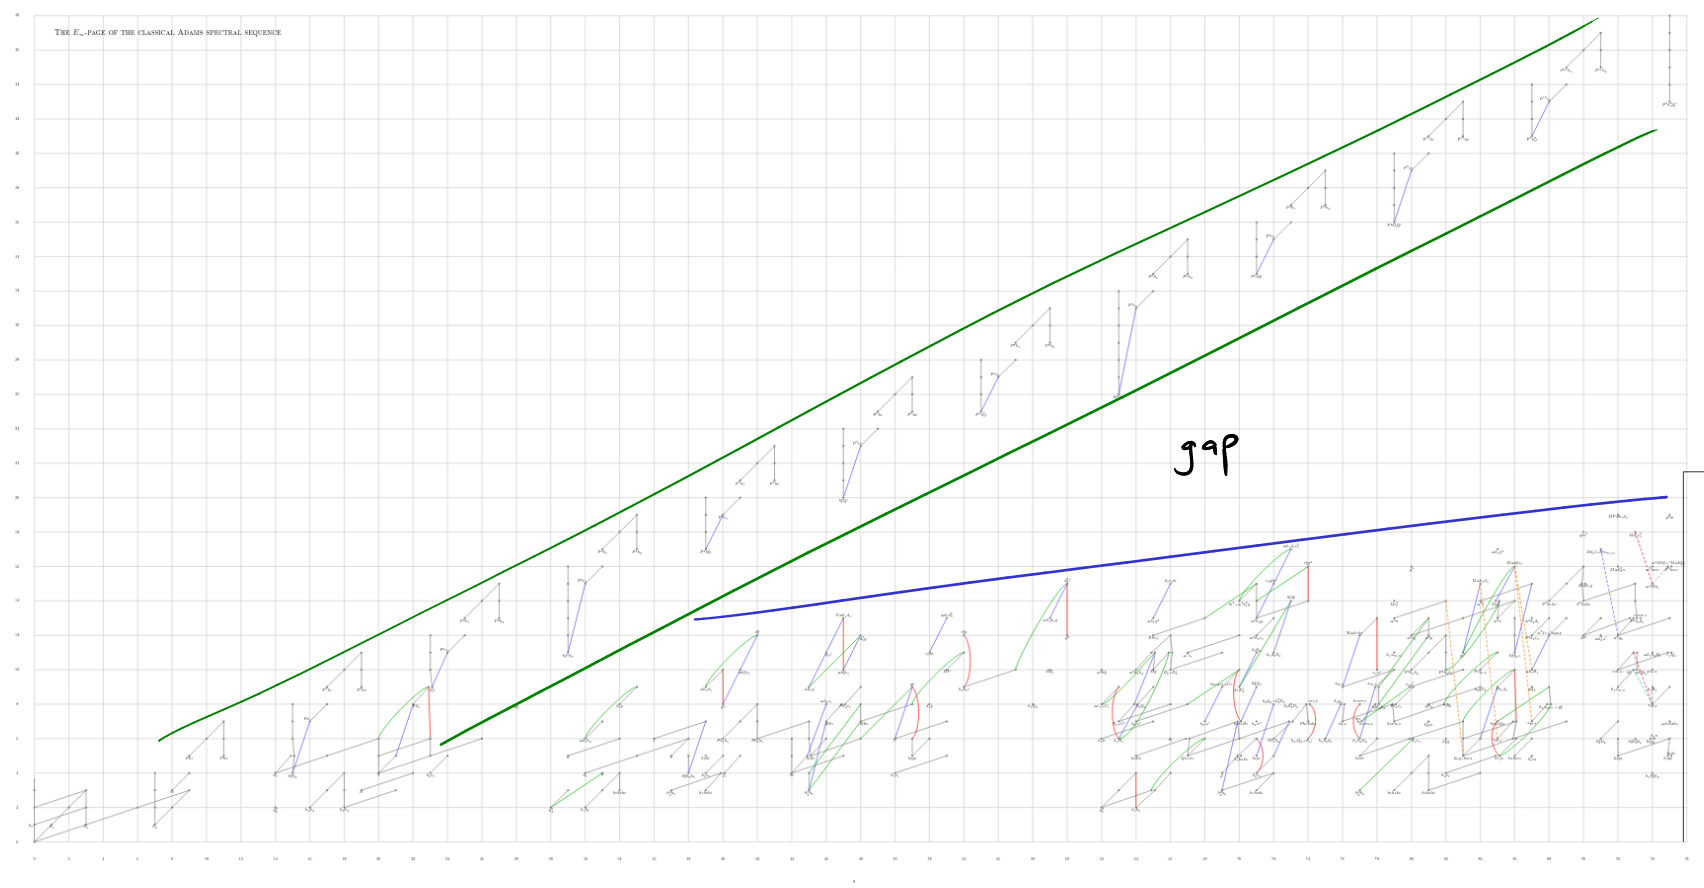
\includegraphics[width=\textwidth]{18_905-201207-6.png}
\end{center}

When we look at the chart, we see that there is a simple collection
of points with larger slope than the rest of the points, indicated with green.
There is also a chaotic pattern of points below it, with a gap in between.

In particular, there are a simple group of homotopy groups
that are hard to detect with homology,
and then there is a messy collection of homotopy groups that
are easier to detect (but still quite hard) with homology.

There is indeed a good understanding of the maps corresponding to
very high Adams filtration, and this region is called
the \(v_1\)-periodic homotopy groups of spheres.
Then there seems to be a gap, and an open problem is
whether this gap continues, and how big it is.
Another natural question is whether we can understand the
non-\(v_1\)-periodic stuff.


\begin{definition}
  An \vocab{extraordinary (co)homology theory} \(E_*\) is a functor % chktex 36
  \[
    E_* \colon \cHoTop \to \text{graded \(\cAb\) groups}
  \]
  satisfying all of the Eilenberg-Steenrod axioms except the dimension axiom.
\end{definition}

They can directly tell, sometimes,
the differences between various maps \(f \colon S^m \to S^n\).
In particular, \(E_*(f) \colon E_*(S^m) \to E_*(S^n)\) could be nontrivial,
because the homologies of a sphere do not have to be
concentrated in one degree.

The most important example is \(E_* = KO_*\),
called \vocab{topological \(K\)-theory}.
This theory sees the \(v_1\)-periodic part of \(\pi_* \mathbb S\).
It has a geometric definition in terms of vector bundles,
which assemble to define \(K\)-theory.
It also has a more algebraic/combinatorial definition.

\begin{question}
  How do we make extraordinary (co)homology theories that detect % chktex 36
  other elements in \(\pi_* \mathbb S\)?
\end{question}

\begin{definition}[Idea]
  An \vocab{\(\mathbb E_\infty\)-ring} is a cohomology theory \(E^*\)
  valued in graded commutative rings.
\end{definition}

For example, we could have \(E^*(X) = H^*(X; R)\),
  where \(R\) is a commutative ring.
We can also have \(E^*(X) = KO^*(X)\).

Given an \(\mathbb E_\infty\)-ring \(E^*\),
we can extract a classical ring, which is \(E^*(*)\).
For example, the classical ring underlying \(H^*({-}; R)\) is
  \(H^*(*; R) \iso R\) in degree \(0\).
On the other hand, the classical ring underlying \(KO^*({-})\) is
  \(KO^*(*)\), which is \(8\)-periodic. (Bott peridicity)

The main idea of algebraic homotopy theory is that we should develop
all of commutative algebra replacing rings with \(\mathbb E_\infty\)-rings.
In particular, wherever we have concepts about rings
like PIDs or Nakayama's lemma, we should try to find an analogous theorem
about \(\mathbb E_\infty\)-rings.
This is what Waldhausen called ``brave new algebra'',
which is today sometimes called ``higher algebra'',
                                ``spectral algebra'', or
                                ``derived algebra''.
A lot of the results we get are the same, but sometimes there are difference.

\begin{example}
  In classical algebra or number theory, people study elliptic curves.
  To imitate the theory of elliptic curves in \(\mathbb E_\infty\)-rings,
  we are led to the notion of \vocab{elliptic cohomology theories}.
\end{example}

One intersecting thing that doesn't happen in classical number theory is that
there is a universal elliptic cohomology theory.
In particular, there is an elliptic cohomology theory that captures the
information of all other elliptic cohomology theories.
This is a new phenomenon that we cannot understand with regular rings.
This universal theory is called \vocab{topological modular forms} (tmf).

We can try to understand the underlying classical ring by
looking at the underlying classical ring \(\mathrm{tmf}^*(*) \otimes_\ZZ \QQ\),
and it turns out to be the classical ring of modular forms.

One can keep going into things like automorphic forms or abelian varieties
and try to construct analogs in this land of brave new algebra.
\(\mathbb E_\infty\)-rings are about commutative algebra,
but we can also talk about associative rings,
which are called \(\mathbb E_1\)- rings.
When we do this, we get a lot of analogs,
and oftentimes we get more objects that we can construct
compared to classical ring theory,
and a lot of the time they are universal.
This is the topic of study in \vocab{chromatic homotopy theory},
which assembles the homotopy groups \(\pi_* \mathbb S\) out of things
detected by \(\mathbb E_\infty\)-rings.
Each \(\mathbb E_\infty\)-ring has a chromatic height that roughly measures
how much of the homotopy group it can see.
\begin{itemize}[nosep]
  \item Height 0 is ordinary homology,
  \item Height 1 is topological \(K\)-theory,
  \item Height 2 is TMF, and so on.
\end{itemize}
Furthermore, we have the chromatic convergence theorem, which says that
each element in \(\pi_* \mathbb S\) is detected at some chromatic height.

Another big open question in this subject is whether
there is a geometric construction of TMF. % chktex 13
For example, we can understand ordinary homology through cycles and
maps of simplices, and we can understand \(K\)-theory with vector bundles.
Physicists tell us that it should be related to the Dirac operator
on the space of loops in \(X\).
However, nobody has been able to do this mathematically in a well defined way.









\end{document}
